\subsection{Examples}
\label{sec:examples}

Another experiment we ran was to evaluate the accuracy of the classifier in a
setting where, if the correct token is not within the top few predictions, the
user types in one or more characters to ``home in'' on the correct prediction.
Figure~\ref{fig:codeexample} shows the results for this experiment. In this
experiment, a character is colored in green if the token is correctly predicted
(i.e., top prediction) before that character is typed. It is colored in yellow
if the token is among the top 5 before typing that character, and colored in red
if the token is not among the top 5. So, for example, in the first
{\tt int} the character {\tt i} is in yellow since before typing {\tt i}, the
token {\tt int} was among the top 5. After typing {\tt i}, the top prediction
was {\tt int}, and thus the characters {\tt n} and {\tt t} are both in green. We
can see that, for example, entire sequences of code such as {\tt if (rc) return
rc;} are predicted correctly without typing anything.
\begin{figure}[h]
  \centering
  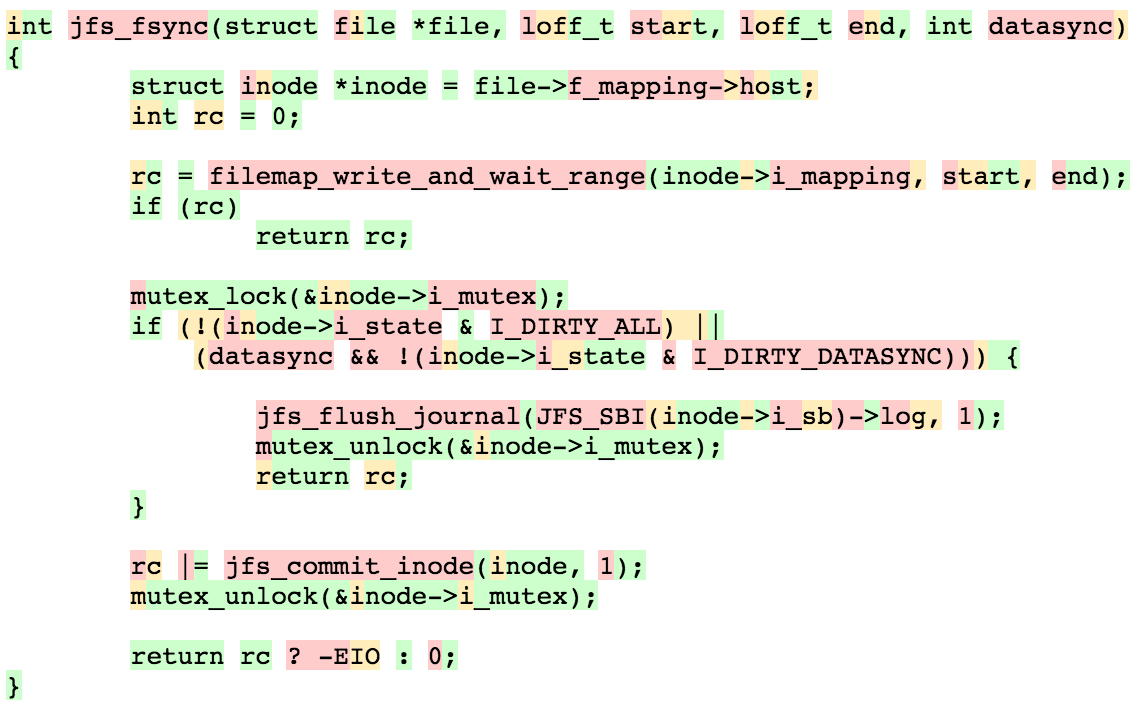
\includegraphics[width=\linewidth]{figs/code_example.png}
  \caption{Code example with per-character predictions}
  \label{fig:codeexample}
\end{figure}

